\documentclass[10pt,twocolumn,a4paper]{article}

% ── Packages ──────────────────────────────────────────────────────────
\usepackage[T1]{fontenc}
\usepackage[utf8]{inputenc}
\usepackage[english]{babel}
\usepackage[top=2.2cm, bottom=2.4cm,
            left=1.65cm, right=1.65cm,
            columnsep=0.55cm,
            headheight=13pt]{geometry}

\usepackage{amsmath,amssymb,amsthm}
\usepackage{mathtools}
\usepackage{bm}
\usepackage{booktabs}
\usepackage{tabularx}
\usepackage{array}
\usepackage{multirow}
\usepackage{graphicx}
\usepackage{float}
\usepackage{caption}
\usepackage{xcolor}
\usepackage{setspace}
\usepackage{parskip}
\usepackage{enumitem}
\usepackage{titlesec}
\usepackage{fancyhdr}
\usepackage{authblk}
\usepackage{flushend}
\usepackage{natbib}
\usepackage[hidelinks]{hyperref}
\usepackage{pgfplots}
\pgfplotsset{compat=1.18}
\usetikzlibrary{calc}

% ── Colors ────────────────────────────────────────────────────────────
\definecolor{darkblue}{RGB}{8, 32, 80}
\definecolor{mygray}  {RGB}{100, 100, 100}
\definecolor{darkgray}{RGB}{50, 50, 50}
\definecolor{hairline}{RGB}{180, 190, 210}
\definecolor{stratred} {RGB}{160, 20, 20}
\definecolor{plotblue} {RGB}{8,   80, 160}
\definecolor{plotred}  {RGB}{180,  30,  30}
\definecolor{plotgray} {RGB}{160, 160, 160}
\definecolor{zeroaxis}{RGB}{120, 120, 120}

% ── PGFPlots shared style ─────────────────────────────────────────────
\pgfplotsset{
  pnlstyle/.style={
    width=\columnwidth, height=4.0cm,
    axis lines=center,
    xlabel={$S_T$}, ylabel={$\Pi$},
    xlabel style={right, font=\scriptsize\itshape},
    ylabel style={above, font=\scriptsize\itshape},
    tick label style={font=\tiny},
    xtick=\empty, ytick={0},
    yticklabels={\scriptsize$0$},
    grid=none, clip=false,
    every axis plot/.append style={line width=1.4pt},
    axis line style={color=darkgray, thin},
  }
}

% ── Typography ────────────────────────────────────────────────────────
\setlength{\parskip}{2.5pt plus 1pt}
\setlength{\parindent}{1em}
\frenchspacing

% ── Section titles ────────────────────────────────────────────────────
\titleformat{\section}
  {\normalsize\bfseries\scshape\color{darkblue}}
  {\Roman{section}.}{0.45em}{}
  [{\color{hairline}\vspace{1pt}\noindent\makebox[\hsize]{\rule{\hsize}{0.35pt}}\vspace{1.5pt}}]

\titleformat{\subsection}
  {\small\bfseries\color{darkgray}}
  {\Alph{subsection}.}{0.4em}{}

% Red variant for strategy subsections
\newcommand{\stratheading}[1]{%
  \subsection*{\small\bfseries\color{stratred}#1}%
  \addcontentsline{toc}{subsection}{#1}%
}

% Lettered red subsection for strategies
\newcounter{stratsubsec}[section]
\newcommand{\stratsubsection}[1]{%
  \refstepcounter{stratsubsec}%
  \vspace{5pt plus 1pt}%
  {\noindent\small\bfseries\color{stratred}\Alph{stratsubsec}.\enspace #1}%
  \vspace{2pt}\par%
}

\titleformat{\subsubsection}
  {\small\itshape\color{darkgray}}
  {}{0pt}{}

\titlespacing*{\section}      {0pt}{7pt plus 2pt}{3pt plus 1pt}
\titlespacing*{\subsection}   {0pt}{5pt plus 1pt}{2pt}
\titlespacing*{\subsubsection}{0pt}{3pt}{1pt}

% ── Headers / footers ─────────────────────────────────────────────────
\pagestyle{fancy}
\fancyhf{}
\fancyhead[L]{\footnotesize\itshape\color{mygray}
Options Strategies on SPY}
%\fancyhead[R]{\footnotesize\itshape\color{mygray}Working Paper}
\fancyfoot[C]{\small\color{mygray}\thepage}
\renewcommand{\headrulewidth}{0.3pt}
\renewcommand{\headrule}{%
  \hbox to\headwidth{\color{hairline}\leaders\hrule height\headrulewidth\hfill}}

% ── Caption style ─────────────────────────────────────────────────────
\captionsetup{
  font=footnotesize,
  labelfont={bf,color=darkblue},
  labelsep=period,
  skip=3pt,
  justification=raggedright,
  singlelinecheck=false
}

% ── Float spacing ─────────────────────────────────────────────────────
\setlength{\textfloatsep}{7pt plus 2pt minus 2pt}
\setlength{\floatsep}{5pt}
\setlength{\intextsep}{5pt}
\setlength{\dbltextfloatsep}{8pt plus 2pt minus 2pt}
\setlength{\dblfloatsep}{6pt}

% ── Math macros ───────────────────────────────────────────────────────
\newcommand{\E}{\mathbb{E}}
\newcommand{\dd}{\mathrm{d}}
\newcommand{\sigiv}{\sigma^{\mathrm{IV}}}
\newcommand{\sigrv}{\sigma^{\mathrm{RV}}}
\DeclareMathOperator{\VaR}{VaR}
\DeclareMathOperator{\CVaR}{CVaR}

% ── Theorem environments ──────────────────────────────────────────────
\newtheoremstyle{mydef}
  {4pt}{3pt}{\small}{}
  {\bfseries\color{darkblue}}{.}{ }{}
\theoremstyle{mydef}
\newtheorem{definition}{Definition}

% ─────────────────────────────────────────────────────────────────────
\begin{document}

% ══════════════════════════════════════════════════════════════════════
%  TITLE BLOCK
% ══════════════════════════════════════════════════════════════════════
\twocolumn[{%
\begin{@twocolumnfalse}

  \vspace*{-0.3cm}
  {\color{darkblue}\rule{\linewidth}{1.8pt}}
  \vspace{5pt}

  \begin{center}
    {\LARGE\bfseries\color{darkblue}
      Systematic Options Strategies on the S\&P~500:\\[5pt]
      Buy-Write, Protective Put, Collar,\\[4pt]
      and Long Straddle}

    \vspace{10pt}

    {\large\textbf{Jean Philippe N'Dri}}\\[3pt]
    {\normalsize\textit{Quantitative Researcher}
    \quad\textcolor{mygray}{$|$}\quad 2026}

    \vspace{8pt}
  \end{center}

  {\color{hairline}\rule{\linewidth}{0.6pt}}
  \vspace{10pt}

\end{@twocolumnfalse}
}]

\setcounter{page}{1}

% ══════════════════════════════════════════════════════════════════════
\section{Data}
\label{sec:data}
% ══════════════════════════════════════════════════════════════════════

\subsection{Dataset}

We use a daily end-of-day SPY options dataset covering January~2020 to
December~2022 (782 trading days). The data source is Kaggle. Each row
of the dataset represents the information associated with one strike
price and a given expiration date on a given quote date. Specifically,
each row contains the bid, ask, implied volatility, and delta for both
the call \emph{and} the put at that strike and expiry.

\subsection{Key Columns}

\begin{table}[H]
\centering
\caption{Key columns in the options dataset.}
\label{tab:cols}
\renewcommand{\arraystretch}{1.10}
\setlength{\tabcolsep}{4pt}
\begin{tabular}{ll}
\toprule
\textbf{Column} & \textbf{Description} \\
\midrule
\texttt{QUOTE\_DATE}       & Quotation date \\
\texttt{UNDERLYING\_LAST}  & SPY closing price \\
\texttt{EXPIRE\_DATE}      & Option expiration date \\
\texttt{DTE}               & Days to expiration \\
\texttt{STRIKE}            & Strike price \\
\texttt{C\_DELTA / P\_DELTA} & Call / put delta \\
\texttt{C\_BID, C\_ASK}    & Call bid and ask \\
\texttt{P\_BID, P\_ASK}    & Put bid and ask \\
\texttt{C\_IV / P\_IV}     & Call / put implied volatility \\
\bottomrule
\end{tabular}
\end{table}


% ══════════════════════════════════════════════════════════════════════
\section{Options Strategies: Construction}
\label{sec:strats}
% ══════════════════════════════════════════════════════════════════════

\stratsubsection{Roll Engine}

At each roll date, options are selected by a two-step algorithm:
\textbf{(1)}~find the expiry whose DTE is closest to the target DTE;
\textbf{(2)}~within that expiry, select the strike whose delta is
closest to the target delta. All trades execute at mid-price. Roll
parameters for all four strategies are summarised in
Table~\ref{tab:params}.

\begin{table}[H]
\centering
\caption{Roll parameters for each strategy.}
\label{tab:params}
\renewcommand{\arraystretch}{1.12}
\setlength{\tabcolsep}{4pt}
\begin{tabular}{llccc}
\toprule
\textbf{Strategy} & \textbf{Legs} & \textbf{DTE} & $\bm{\Delta}$ & \textbf{Freq.}\\
\midrule
Buy-Write      & $-C$       & 7  & $+0.50$     & Weekly  \\
Prot.\ Put     & $+P$       & 30 & $-0.30$     & Monthly \\
Collar         & $+P,\;-C$  & 30 & ${\pm}0.25$ & Monthly \\
Long Straddle  & $+C,\;+P$  & 30 & ${\pm}0.50$ & Monthly \\
\bottomrule
\end{tabular}
\end{table}

\stratsubsection{Buy-Write (Covered Call)}

The buy-write holds one unit of SPY and sells one ATM call each week.
The P\&L at expiration is the sum of three components: the change in
the stock position, the premium received, and the settlement of the
short call.

\noindent\textit{Full payoff at expiration} (premium received $c$,
strike $K_c$, entry price $S_0$):
\begin{align}
  \Pi_{\mathrm{BW}}(S_T)
  &= \underbrace{(S_T - S_0)}_{\text{stock P\&L}}
   + \underbrace{c}_{\text{premium}} \notag\\
  &\quad - \underbrace{\max(S_T - K_c,\; 0)}_{\text{short call settlement}}
  \label{eq:bw_full}
\end{align}

Evaluating the two cases explicitly:
\begin{equation}
  \Pi_{\mathrm{BW}}(S_T)=
  \begin{cases}
    S_T - S_0 + c              & S_T \leq K_c,\\[2pt]
    K_c - S_0 + c              & S_T > K_c.
  \end{cases}
  \label{eq:bw}
\end{equation}

Maximum gain is capped at $K_c - S_0 + c$; the break-even is
$S_0 - c$.

% S0=100, Kc=102, c=2 => BE=98, max gain=4
\begin{figure}[H]
\centering
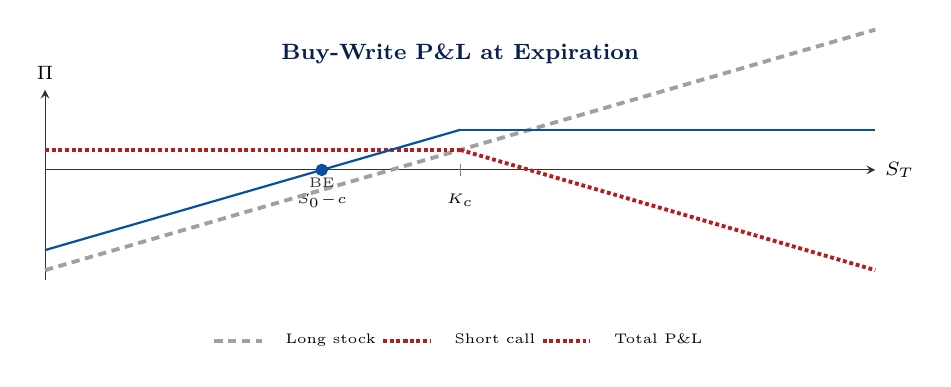
\begin{tikzpicture}
\begin{axis}[pnlstyle,
  xmin=90, xmax=114, ymin=-11, ymax=8,
  extra x ticks={98,102},
  extra x tick labels={$S_0\!-\!c$,$K_c$},
  extra x tick style={font=\tiny,tick label style={yshift=-3pt}},
  title={\footnotesize\bfseries\color{darkblue}Buy-Write P\&L at Expiration},
  legend columns=3,
  legend style={
    at={(0.5,-0.22)}, anchor=north,
    font=\tiny, draw=none, fill=none,
    column sep=6pt, /tikz/every even column/.append style={column sep=0pt},
  },
]
\addplot[plotgray, densely dashed, domain=90:114] {x - 100};
\addlegendentry{Long stock}
\addplot[plotred, densely dotted, domain=90:102]  {2};
\addplot[plotred, densely dotted, domain=102:114] {2-(x-102)};
\addlegendentry{Short call}
\addplot[plotblue, thick, domain=90:102]  {x - 98};
\addplot[plotblue, thick, domain=102:114] {4};
\addlegendentry{Total P\&L}
\addplot[plotblue,only marks,mark=*,mark size=1.5pt] coordinates{(98,0)};
\node[font=\tiny,darkgray,anchor=north] at (axis cs:98,0.15) {BE};
\end{axis}
\end{tikzpicture}
\caption{Buy-write: long stock $+$ short call. Cap at $K_c-S_0+c$, break-even at $S_0-c$.}
\label{fig:pnl_bw}
\end{figure}

\stratsubsection{Protective Put}

The protective put holds one unit of SPY and buys one OTM put each
month, establishing a floor on portfolio value.  The P\&L at
expiration combines the stock move, the premium paid, and the
settlement of the long put.

\noindent\textit{Full payoff at expiration}:
\begin{align}
  \Pi_{\mathrm{PP}}(S_T)
  &= \underbrace{(S_T - S_0)}_{\text{stock P\&L}}
   - \underbrace{p}_{\text{premium}} \notag\\
  &\quad + \underbrace{\max(K_p - S_T,\; 0)}_{\text{long put settlement}}
  \label{eq:pp_full}
\end{align}

Collecting terms:
\begin{equation}
  \Pi_{\mathrm{PP}}(S_T) =
  \begin{cases}
    K_p - S_0 - p & S_T < K_p,\\[2pt]
    S_T - S_0 - p & S_T \geq K_p.
  \end{cases}
  \label{eq:pp}
\end{equation}

Maximum loss is bounded at $K_p - S_0 - p$; upside is unlimited net
of the premium drag.

% S0=100, Kp=97, p=2 => BE=102, floor=-5
\begin{figure}[H]
\centering
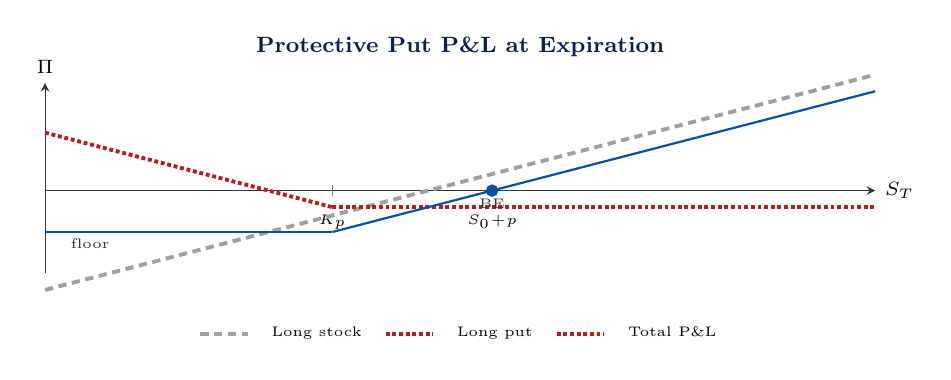
\begin{tikzpicture}
\begin{axis}[pnlstyle,
  xmin=88, xmax=114, ymin=-10, ymax=13,
  extra x ticks={97,102},
  extra x tick labels={$K_p$,$S_0\!+\!p$},
  extra x tick style={font=\tiny,tick label style={yshift=-3pt}},
  title={\footnotesize\bfseries\color{darkblue}Protective Put P\&L at Expiration},
  legend columns=3,
  legend style={
    at={(0.5,-0.22)}, anchor=north,
    font=\tiny, draw=none, fill=none,
    column sep=6pt,
  },
]
\addplot[plotgray, densely dashed, domain=88:114] {x - 100};
\addlegendentry{Long stock}
\addplot[plotred, densely dotted, domain=88:97]  {97 - x - 2};
\addplot[plotred, densely dotted, domain=97:114] {-2};
\addlegendentry{Long put}
\addplot[plotblue, thick, domain=88:97]  {-5};
\addplot[plotblue, thick, domain=97:114] {x - 102};
\addlegendentry{Total P\&L}
\addplot[plotblue,only marks,mark=*,mark size=1.5pt] coordinates{(102,0)};
\node[font=\tiny,darkgray,anchor=north] at (axis cs:102,0.15) {BE};
\node[font=\tiny,darkgray,anchor=north west] at (axis cs:88.5,-4.6) {floor};
\end{axis}
\end{tikzpicture}
\caption{Protective put: long stock $+$ long put. Floor at $K_p-S_0-p$, break-even at $S_0+p$.}
\label{fig:pnl_pp}
\end{figure}

\stratsubsection{Collar}

The collar augments the protective put with a short OTM call, using
the call premium to offset the cost of the put.

\noindent\textit{Full payoff at expiration} (put premium $p$, call
premium $c$, net cost $\delta = p - c$):
\begin{align}
  \Pi_{\mathrm{COL}}(S_T)
  &= \underbrace{(S_T - S_0)}_{\text{stock P\&L}}
   - \underbrace{\delta}_{\text{net premium}} \notag\\
  &\quad + \underbrace{\max(K_p - S_T,\; 0)}_{\text{long put}}
   - \underbrace{\max(S_T - K_c,\; 0)}_{\text{short call}}
  \label{eq:collar_full}
\end{align}

Evaluating the three cases explicitly:
\begin{equation}
  \Pi_{\mathrm{COL}}(S_T)=
  \begin{cases}
    K_p - S_0 - \delta & S_T < K_p,     \\[2pt]
    S_T - S_0 - \delta & K_p \leq S_T \leq K_c, \\[2pt]
    K_c - S_0 - \delta & S_T > K_c.
  \end{cases}
  \label{eq:collar}
\end{equation}

Both profit and loss are bounded.

% S0=100, Kp=97, Kc=103, delta=0 => BE=100
\begin{figure}[H]
\centering
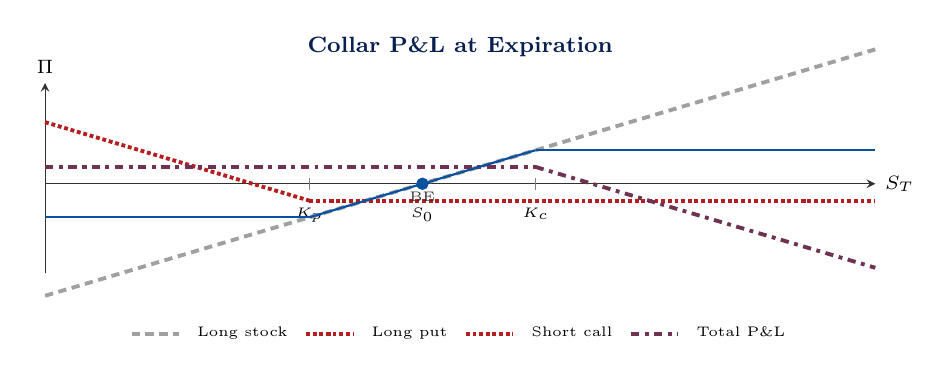
\begin{tikzpicture}
\begin{axis}[pnlstyle,
  xmin=90, xmax=112, ymin=-8, ymax=9,
  extra x ticks={97,100,103},
  extra x tick labels={$K_p$,$S_0$,$K_c$},
  extra x tick style={font=\tiny,tick label style={yshift=-3pt}},
  title={\footnotesize\bfseries\color{darkblue}Collar P\&L at Expiration},
  legend columns=4,
  legend style={
    at={(0.5,-0.22)}, anchor=north,
    font=\tiny, draw=none, fill=none,
    column sep=4pt,
  },
]
\addplot[plotgray, densely dashed, domain=90:112] {x - 100};
\addlegendentry{Long stock}
\addplot[plotred, densely dotted, domain=90:97]  {97 - x - 1.5};
\addplot[plotred, densely dotted, domain=97:112] {-1.5};
\addlegendentry{Long put}
\addplot[plotred!60!plotblue, dash dot, domain=90:103]  {1.5};
\addplot[plotred!60!plotblue, dash dot, domain=103:112] {1.5-(x-103)};
\addlegendentry{Short call}
\addplot[plotblue, thick, domain=90:97]  {-3};
\addplot[plotblue, thick, domain=97:103] {x - 100};
\addplot[plotblue, thick, domain=103:112]{3};
\addlegendentry{Total P\&L}
\addplot[plotblue,only marks,mark=*,mark size=1.5pt] coordinates{(100,0)};
\node[font=\tiny,darkgray,anchor=north] at (axis cs:100,0.15) {BE};
\end{axis}
\end{tikzpicture}
\caption{Collar: long stock $+$ long put $+$ short call. Floor and cap both bounded.}
\label{fig:pnl_collar}
\end{figure}

\stratsubsection{Long Straddle}

The long straddle buys both the ATM call and the ATM put with no
underlying position. It is a direction-neutral bet that the realized
move will exceed the implied move.

\noindent\textit{Full payoff at expiration}:
\begin{align}
  \Pi_{\mathrm{LS}}(S_T)
  &= \underbrace{\max(S_T - K,\; 0)}_{\text{long call}}
   + \underbrace{\max(K - S_T,\; 0)}_{\text{long put}} \notag\\
  &\quad - \underbrace{(c + p)}_{\text{total premium}}
  \label{eq:straddle_full}
\end{align}

Since exactly one of the two max terms is positive (or both are zero
when $S_T = K$), this simplifies to:
\begin{equation}
  \Pi_{\mathrm{LS}}(S_T) = |S_T - K| - (c + p)
  \label{eq:straddle}
\end{equation}

Break-even points are $K \pm (c+p)$.

The strategy is profitable if and only if $\sigrv > \sigiv$.

% K=100, c=2.5, p=2.5 => c+p=5, BE at 95 and 105
\begin{figure}[H]
\centering
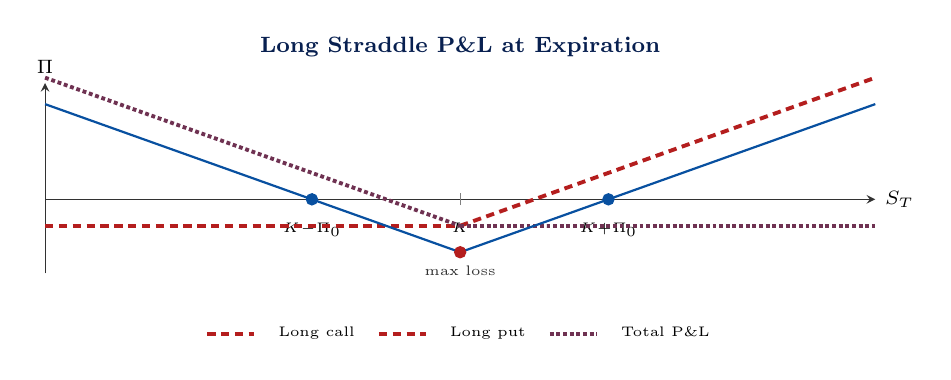
\begin{tikzpicture}
\begin{axis}[pnlstyle,
  xmin=86, xmax=114, ymin=-7, ymax=11,
  extra x ticks={95,100,105},
  extra x tick labels={$K\!-\!\Pi_0$,$K$,$K\!+\!\Pi_0$},
  extra x tick style={font=\tiny,tick label style={yshift=-3pt}},
  title={\footnotesize\bfseries\color{darkblue}Long Straddle P\&L at Expiration},
  legend columns=3,
  legend style={
    at={(0.5,-0.22)}, anchor=north,
    font=\tiny, draw=none, fill=none,
    column sep=6pt,
  },
]
\addplot[plotred, densely dashed, domain=86:100]  {-2.5};
\addplot[plotred, densely dashed, domain=100:114] {x - 102.5};
\addlegendentry{Long call}
\addplot[plotred!60!plotblue, densely dotted, domain=86:100]  {97.5 - x};
\addplot[plotred!60!plotblue, densely dotted, domain=100:114] {-2.5};
\addlegendentry{Long put}
\addplot[plotblue, thick, domain=86:100]  {95 - x};
\addplot[plotblue, thick, domain=100:114] {x - 105};
\addlegendentry{Total P\&L}
\addplot[plotred,only marks,mark=*,mark size=1.5pt] coordinates{(100,-5)};
\addplot[plotblue,only marks,mark=*,mark size=1.5pt] coordinates{(95,0)(105,0)};
\node[font=\tiny,darkgray,anchor=north] at (axis cs:100,-5.4) {max loss};
\end{axis}
\end{tikzpicture}
\caption{Long straddle: long call $+$ long put. Max loss $-(c+p)$ at $K$, break-evens at $K\pm(c+p)$.}
\label{fig:pnl_ls}
\end{figure}
\label{sec:index}
% ══════════════════════════════════════════════════════════════════════

\stratsubsection{Daily Portfolio Valuation}

Each strategy is represented as a daily index rebased to 100 at
inception. The general form of the daily portfolio value $V_t$ differs
by strategy:

\begin{align}
  V_t^{\mathrm{BW}}  &= S_t + \mathrm{Cash}_t - C_t^{\mathrm{MTM}}
  \label{eq:v_bw}\\
  V_t^{\mathrm{PP}}  &= S_t + \mathrm{Cash}_t + P_t^{\mathrm{MTM}}
  \label{eq:v_pp}\\
  V_t^{\mathrm{COL}} &= S_t + \mathrm{Cash}_t
                        + P_t^{\mathrm{MTM}} - C_t^{\mathrm{MTM}}
  \label{eq:v_col}\\
  V_t^{\mathrm{LS}}  &= \mathrm{Cash}_t
                        + C_t^{\mathrm{MTM}} + P_t^{\mathrm{MTM}}
  \label{eq:v_ls}
\end{align}

where $C_t^{\mathrm{MTM}}$ and $P_t^{\mathrm{MTM}}$ are the daily
mid-price values of the open call and put positions respectively.

\stratsubsection{Cash Account}

The cash account $\mathrm{Cash}_t$ accumulates all premium flows:
\begin{itemize}[leftmargin=1.4em, itemsep=1pt, topsep=2pt]
  \item \textbf{At roll:} cash receives (for sold legs) or pays
    (for bought legs) the mid-price premium.
  \item \textbf{At expiration:} cash is debited by the intrinsic value
    of any short leg that expires in-the-money, or credited by the
    intrinsic of any long leg.
\end{itemize}

Formally, for a short call at strike $K_c$:
\begin{equation}
  \mathrm{Cash}_{\mathrm{expiry}} \mathrel{-}=
  \max(S_T - K_c,\; 0)
  \label{eq:settle_call}
\end{equation}

and for a long put at strike $K_p$:
\begin{equation}
  \mathrm{Cash}_{\mathrm{expiry}} \mathrel{+}=
  \max(K_p - S_T,\; 0)
  \label{eq:settle_put}
\end{equation}

\stratsubsection{Index Level}

The strategy index is defined as:
\begin{equation}
  I_t = 100 \times \frac{V_t}{V_0}
  \label{eq:index}
\end{equation}

where $V_0$ is the portfolio value on the first trading day. For
comparison, the SPY buy-and-hold index is:
\begin{equation}
  I_t^{\mathrm{SPY}} = 100 \times \frac{S_t}{S_0}
  \label{eq:spy_bnh}
\end{equation}

Rebasing both series to 100 at $t=0$ allows direct visual comparison
of cumulative returns regardless of the absolute dollar value of the
initial portfolio.

\stratsubsection{Settlement and Roll Timing}

Expiration and roll occur on the \emph{same} trading day:
\begin{enumerate}[leftmargin=1.6em, itemsep=1pt, topsep=2pt]
  \item Settle the expiring position using the end-of-day SPY price.
  \item Immediately sell (or buy) the new option using end-of-day
    mid-prices on the same date.
\end{enumerate}

This same-day roll is operationally realistic: SPY weekly options
expire at the open on Friday, and a new position can be opened before
the 16:00 close. The settlement condition uses strict equality:
\begin{equation}
  \texttt{current\_expiry} == \texttt{date}
  \label{eq:settle_cond}
\end{equation}
to avoid double-settlement on days when the position is already closed.

\stratsubsection{Look-Ahead Bias}

The backtest is free of look-ahead bias. All prices used on date $t$
are sourced exclusively from the end-of-day snapshot of date $t$:
option selection, execution, and mark-to-market all use the same
16:00 cross-section. The only modest optimism is mid-price execution,
which assumes fills exactly at the midpoint of the bid-ask spread.


% ══════════════════════════════════════════════════════════════════════
\section{Performance Metrics}
\label{sec:metrics}
% ══════════════════════════════════════════════════════════════════════

Let $\{r_t\}_{t=1}^{n}$ denote the daily returns of strategy index
$I_t$, with $r_t = I_t / I_{t-1} - 1$.

\subsection{Return and Volatility}

\begin{align}
  \mu_{\mathrm{ann}} &=
    \Bigl(\prod_{t=1}^{n}(1+r_t)\Bigr)^{252/n} - 1
  \label{eq:ann_ret}\\[3pt]
  \sigma_{\mathrm{ann}} &= \hat\sigma(r)\cdot\sqrt{252}
  \label{eq:ann_vol}
\end{align}

\subsection{Risk-Adjusted Ratios}

The Sharpe ratio measures excess return per unit of total volatility:
\begin{equation}
  \text{Sharpe} = \frac{\mu_{\mathrm{ann}}}{\sigma_{\mathrm{ann}}}
  \label{eq:sharpe}
\end{equation}

The Sortino ratio penalises only downside deviations, making it more
appropriate for strategies with asymmetric return distributions:
\begin{equation}
  \text{Sortino} = \frac{\mu_{\mathrm{ann}}}
                        {\sigma_{\mathrm{down}}\cdot\sqrt{252}}
  \label{eq:sortino}
\end{equation}

where $\sigma_{\mathrm{down}} = \mathrm{std}(r_t \mid r_t < 0)$.

The Calmar ratio relates annualised return to the maximum loss ever
sustained:
\begin{equation}
  \text{Calmar} = \frac{\mu_{\mathrm{ann}}}{|\mathrm{MaxDD}|}
  \label{eq:calmar}
\end{equation}

The Omega ratio measures the ratio of gains to losses relative to a
threshold (here zero), capturing the full shape of the distribution:
\begin{equation}
  \text{Omega} = \frac{\displaystyle\sum_{r_t>0} r_t}
                      {\displaystyle\bigl|\sum_{r_t<0} r_t\bigr|}
  \label{eq:omega}
\end{equation}

\subsection{Drawdown}

The drawdown at date $t$ measures the percentage decline from the
running peak:
\begin{equation}
  \mathrm{DD}_t =
    \frac{I_t - \max_{s \leq t}\,I_s}{\max_{s \leq t}\,I_s}
  \label{eq:dd}
\end{equation}

The maximum drawdown is $\mathrm{MaxDD} = \min_t\,\mathrm{DD}_t$.

\subsection{Tail Risk}

Value-at-Risk at the 95\% confidence level gives the loss threshold
exceeded on only 5\% of days:
\begin{equation}
  \VaR_{95\%} = -\,\mathrm{percentile}(r,\; 5\%)
  \label{eq:var}
\end{equation}

Conditional Value-at-Risk (CVaR), also known as Expected Shortfall,
is the average loss on the worst 5\% of days:
\begin{equation}
  \CVaR_{95\%} = -\,\E\bigl[r \;\big|\; r \leq -\VaR_{95\%}\bigr]
  \label{eq:cvar}
\end{equation}

CVaR is a coherent risk measure \citep{artzner_1999} and is
particularly informative for option strategies whose return
distributions exhibit significant skewness and excess kurtosis.

% ── References ────────────────────────────────────────────────────────

\end{document}